\documentclass[a4paper, 12pt]{article}

% packages
\usepackage{amssymb}
\usepackage[fleqn]{mathtools}
\usepackage{tikz}
\usepackage{enumerate}
\usepackage{bussproofs}
\usepackage{xcolor}
\usepackage[margin=1.3cm]{geometry}
\usepackage{logicproof}
\usepackage{diagbox}
\usepackage{listings}
\usepackage{graphicx}
\usepackage{lstautogobble}
\usepackage{hyperref}
\usepackage{multirow}
\usepackage{tipa}
\usepackage{pgfplots}
\usepackage{adjustbox}

% tikz libraries
\usetikzlibrary{
    decorations.pathreplacing,
    arrows,
    shapes,
    shapes.gates.logic.US,
    circuits.logic.US,
    calc,
    automata,
    positioning,
    intersections
}

\pgfplotsset{compat=1.16}

\pgfmathdeclarefunction{gauss}{2}{%
  \pgfmathparse{1/(#2*sqrt(2*pi))*exp(-((x-#1)^2)/(2*#2^2))}%
}

\allowdisplaybreaks % allow environments to break
\setlength\parindent{0pt} % no indent

% shorthand for verbatim
% this clashes with logicproof, so maybe fix this at some point?
\catcode`~=\active
\def~#1~{\texttt{#1}}

% code listing
\lstdefinestyle{main}{
    numberstyle=\tiny,
    breaklines=true,
    showspaces=false,
    showstringspaces=false,
    tabsize=2,
    numbers=left,
    basicstyle=\ttfamily,
    columns=fixed,
    fontadjust=true,
    basewidth=0.5em,
    autogobble,
    xleftmargin=3.0ex,
    mathescape=true
}
\newcommand{\dollar}{\mbox{\textdollar}} %
\lstset{style=main}

% augmented matrix
\makeatletter
\renewcommand*\env@matrix[1][*\c@MaxMatrixCols c]{%
\hskip -\arraycolsep
\let\@ifnextchar\new@ifnextchar
\array{#1}}
\makeatother

% ceiling / floor
\DeclarePairedDelimiter{\ceil}{\lceil}{\rceil}
\DeclarePairedDelimiter{\floor}{\lfloor}{\rfloor}

% custom commands
\newcommand{\indefint}[2]{\int #1 \, \mathrm{d}#2}
\newcommand{\defint}[4]{\int_{#1}^{#2} #3 \, \mathrm{d}#4}
\newcommand{\pdif}[2]{\frac{\partial #1}{\partial #2}}
\newcommand{\dif}[2]{\frac{\mathrm{d}#1}{\mathrm{d}#2}}
\newcommand{\limit}[2]{\raisebox{0.5ex}{\scalebox{0.8}{$\displaystyle{\lim_{#1 \to #2}}$}}}
\newcommand{\limitsup}[2]{\raisebox{0.5ex}{\scalebox{0.8}{$\displaystyle{\limsup_{#1 \to #2}}$}}}
\newcommand{\summation}[2]{\sum\limits_{#1}^{#2}}
\newcommand{\product}[2]{\prod\limits_{#1}^{#2}}
\newcommand{\intbracket}[3]{\left[#3\right]_{#1}^{#2}}
\newcommand{\laplace}{\mathcal{L}}
\newcommand{\fourier}{\mathcal{F}}
\newcommand{\mat}[1]{\boldsymbol{#1}}
\renewcommand{\vec}[1]{\boldsymbol{#1}}
\newcommand{\rowt}[1]{\begin{bmatrix}
    #1
\end{bmatrix}^\top}
\DeclareMathOperator*{\argmax}{argmax}
\DeclareMathOperator*{\argmin}{argmin}

\newcommand{\lto}[0]{\leadsto\ }

\newcommand{\ulsmash}[1]{\underline{\smash{#1}}}

\newcommand{\powerset}[0]{\wp}
\renewcommand{\emptyset}[0]{\varnothing}

\makeatletter
\newsavebox{\@brx}
\newcommand{\llangle}[1][]{\savebox{\@brx}{\(\m@th{#1\langle}\)}%
  \mathopen{\copy\@brx\kern-0.5\wd\@brx\usebox{\@brx}}}
\newcommand{\rrangle}[1][]{\savebox{\@brx}{\(\m@th{#1\rangle}\)}%
  \mathclose{\copy\@brx\kern-0.5\wd\@brx\usebox{\@brx}}}
\makeatother
\newcommand{\lla}{\llangle}
\newcommand{\rra}{\rrangle}
\newcommand{\la}{\langle}
\newcommand{\ra}{\rangle}
\newcommand{\crnr}[1]{\text{\textopencorner} #1 \text{\textcorner}}
\newcommand{\bnfsep}[0]{\ |\ }
\newcommand{\concsep}[0]{\ ||\ }

\newcommand{\axiom}[1]{\AxiomC{#1}}
\newcommand{\unary}[1]{\UnaryInfC{#1}}
\newcommand{\binary}[1]{\BinaryInfC{#1}}
\newcommand{\trinary}[1]{\TrinaryInfC{#1}}
\newcommand{\quaternary}[1]{\QuaternaryInfC{#1}}
\newcommand{\quinary}[1]{\QuinaryInfC{#1}}
\newcommand{\dproof}[0]{\DisplayProof}
\newcommand{\llabel}[1]{\LeftLabel{\scriptsize #1}}
\newcommand{\rlabel}[1]{\RightLabel{\scriptsize #1}}

\newcommand{\ttbs}{\char`\\}
\newcommand{\lrbt}[0]{\ \bullet\ }

% colours
\newcommand{\violet}[1]{\textcolor{violet}{#1}}
\newcommand{\blue}[1]{\textcolor{blue}{#1}}
\newcommand{\red}[1]{\textcolor{red}{#1}}
\newcommand{\teal}[1]{\textcolor{teal}{#1}}

% reasoning proofs
\usepackage{ltablex}
\usepackage{environ}
\keepXColumns
\NewEnviron{reasoning}{
    \begin{tabularx}{\textwidth}{rlX}
        \BODY
    \end{tabularx}
}
\newcommand{\proofline}[3]{$(#1)$ & $#2$ & \hfill #3 \smallskip \\}
\newcommand{\proofarbitrary}[1]{& take arbitrary $#1$ \smallskip \\}
\newcommand{\prooftext}[1]{\multicolumn{3}{l}{#1} \smallskip \\}
\newcommand{\proofmath}[3]{$#1$ & = $#2$ & \hfill #3 \smallskip \\}
\newcommand{\prooftherefore}[1]{& $\therefore #1$ \smallskip \\}
\newcommand{\proofbc}[0]{\prooftext{\textbf{Base Case}}}
\newcommand{\proofis}[0]{\prooftext{\textbf{Inductive Step}}}

% ER diagrams
\newcommand{\nattribute}[4]{
    \node[draw, state, inner sep=0cm, minimum size=0.2cm, label=#3:{#4}] (#1) at (#2) {};
}
\newcommand{\mattribute}[4]{
    \node[draw, state, accepting, inner sep=0cm, minimum size=0.2cm, label=#3:{#4}] (#1) at (#2) {};
}
\newcommand{\dattribute}[4]{
    \node[draw, state, dashed, inner sep=0cm, minimum size=0.2cm, label=#3:{#4}] (#1) at (#2) {};
}
\newcommand{\entity}[3]{
    \node[] (#1-c) at (#2) {#3};
    \node[inner sep=0cm] (#1-l) at ($(#1-c) + (-1, 0)$) {};
    \node[inner sep=0cm] (#1-r) at ($(#1-c) + (1, 0)$) {};
    \node[inner sep=0cm] (#1-u) at ($(#1-c) + (0, 0.5)$) {};
    \node[inner sep=0cm] (#1-d) at ($(#1-c) + (0, -0.5)$) {};
    \draw
    ($(#1-c) + (-1, 0.5)$) -- ($(#1-c) + (1, 0.5)$) -- ($(#1-c) + (1, -0.5)$) -- ($(#1-c) + (-1, -0.5)$) -- cycle;
}
\newcommand{\relationship}[3]{
    \node[] (#1-c) at (#2) {#3};
    \node[inner sep=0cm] (#1-l) at ($(#1-c) + (-1, 0)$) {};
    \node[inner sep=0cm] (#1-r) at ($(#1-c) + (1, 0)$) {};
    \node[inner sep=0cm] (#1-u) at ($(#1-c) + (0, 1)$) {};
    \node[inner sep=0cm] (#1-d) at ($(#1-c) + (0, -1)$) {};
    \draw
    ($(#1-c) + (-1, 0)$) -- ($(#1-c) + (0, 1)$) -- ($(#1-c) + (1, 0)$) -- ($(#1-c) + (0, -1)$) -- cycle;
}

% AVL Trees
\newcommand{\avltri}[4]{
    \draw ($(#1)$) -- ($(#1) + #4*(0.5, -1)$) -- ($(#1) + #4*(-0.5, -1)$) -- cycle;
    \node at ($(#1) + #4*(0, -1) + (0, 0.5)$) {#3};
    \node at ($(#1) + #4*(0, -1) + (0, -0.5)$) {#2};
}

% RB Trees
\tikzset{rbtr/.style={inner sep=2pt, circle, draw=black, fill=red}}
\tikzset{rbtb/.style={inner sep=2pt, circle, draw=black, fill=black}}

% Samples
\tikzset{spos/.style={inner sep=2pt, circle, draw=black, fill=blue!20}}
\tikzset{sneg/.style={inner sep=2pt, circle, draw=black, fill=red!20}}

% Joins
\newcommand\ljoin{\stackrel{\mathclap{\normalfont\mbox{\tiny L}}}{\bowtie}}
\newcommand\rjoin{\stackrel{\mathclap{\normalfont\mbox{\tiny R}}}{\bowtie}}
\newcommand\ojoin{\stackrel{\mathclap{\normalfont\mbox{\tiny O}}}{\bowtie}}

\setcounter{MaxMatrixCols}{100}

% actual document
\begin{document}
    {\sc Computing $3^\text{rd}$ Year Notes} \hfill ~https://github.com/lin-e/imperial-revision~
    \rule{\textwidth}{0.1pt}
    \section*{CO331 - Network and Web Security \hfill (60015)}
        \subsection*{Week 1}
            \subsubsection*{Vulnerabilities}
                We define \textbf{vulnerabilities} as bugs or design flaws in software that can be exploited by attackers to compromise computers.
                These are taken advantage of by \textbf{exploits}, which are pieces of software.
                If it is unknown to the software vendor, it is referred to as a \textbf{zero day} (has not been disclosed to the public domain).
                \medskip

                \textbf{Advisories} are used to publicly disclose new vulnerabilities, issued by vendors or security companies.
                These are important for developers, sysadmins as well as regular users of the software, in order to keep up to date or patch systems.
                \medskip

                The \textbf{vulnerability reports} often vary in format.
                Bugs and systems can differ from each other, as well as researchers putting in varying levels of effort.
                Generally, the key information consists of the affected systems, descriptions, impact, proof of concept code, as well as proposed fixes.
                \medskip

                There are a number of approaches for when vulnerabilities are discovered;
                \begin{itemize}
                    \itemsep0em
                    \item \textbf{non-disclosure} \hfill keep the vulnerability secret
                        \smallskip

                        This is preferred by vendors who choose not to use resources to fix bugs (based on `security by obscurity'), or by parties intending to exploit it.
                        \medskip

                        An issue with hoarding vulnerabilities is the accidental release.
                        For example, \textit{WannaCry} used two exploits hoarded by the NSA - if this was disclosed, many more systems may have been patched.
                    \item \textbf{responsible disclosure} \hfill affected vendor decides when and what to release
                        \smallskip

                        This approach is preferred by software vendors, motivated by the idea that end users will not develop their own fixes.
                        However this can lead to a long duration between a discovery and fix.
                    \item \textbf{full disclosure} \hfill make details public
                        \smallskip

                        Eliminates any asymmetric information advantage attackers may have.
                        This method is preferred by security researchers, as well as the open source community.
                        However, it may affect users to attacks.
                        \medskip

                        The current approach, spearheaded by \textit{Google Project Zero}, is to give a window of time to vendors to fix vulnerabilities before it is publicly disclosed.
                \end{itemize}
            \subsubsection*{Malware}
                Malicious software can be characterised by infection vector;
                \begin{itemize}
                    \itemsep0em
                    \item \textbf{virus} \hfill malicious code copying into existing programs
                    \item \textbf{worm} \hfill replicates program over network or removable devices
                    \item \textbf{trojan / spoofed software} \hfill provides (or pretends to) useful service to act legitimate
                    \item \textbf{drive-by download} \hfill code executed by visiting malicious website
                \end{itemize}
                Another way to characterise malware is by purpose (malware often has multiple of these working together);
                \begin{itemize}
                    \itemsep0em
                    \item \textbf{rootkit} \hfill strongest, works at OS level (can hide itself)
                    \item \textbf{backdoor} \hfill allows attackers to connect over network
                    \item \textbf{RAT (remote access tool)} \hfill remote control
                    \item \textbf{botnet} \hfill recruit machine into botnet
                    \item \textbf{keylogger} \hfill logs keystrokes
                    \item \textbf{spyware} \hfill steals sensitive documents
                    \item \textbf{ransomware} \hfill blocks access to machine or data until ransom is paid
                    \item \textbf{cryptominer} \hfill uses system resources to mine cryptocurrency
                    \item \textbf{adware} \hfill displays advertisements
                \end{itemize}
                Malware can exist in several formats;
                \begin{itemize}
                    \itemsep0em
                    \item injected code added to a legitimate program
                    \item library loaded by a legitimate program
                    \item scripts run by application (such as macros in \textit{Microsoft Office})
                    \item standalone executable run by the user
                    \item code loaded in volatile memory (fileless malware) - without a file, detection can be difficult
                \end{itemize}
                Viruses can propagate in a number of ways, either by the attacker in the case of self-replication, or drive-by downloads, or installed by the user, either through social engineering or compromised certificates (in fake software updates).
                \medskip

                A virus can have varying privileges, either from the lowest level (in a rootkit, where it owns the machine), or have user privileges which can do limited damage.
                \medskip

                \textbf{APTs (Advanced Persistent Threats)} are used to reach high-value victims.
                These attacks are specific to the victim, often driven by a human.
                Decisions are made, depending on the specific configurations, and can involve compromising intermediate systems to reach the victim.
                Detection is avoided, with the use of rootkits to hide presence, as well as large datasets being exfiltrated over a long period of time.
                Avoiding detection is important as these attacks are often done over a long period of time, waiting for information to enter the system, as well as retaining access for later use.
                \medskip

                On the other hand, \textbf{botnets} are generic attacks, which aim to infect as many machines as possible.
                The idea is to infect many machines (bots) to allow an attacker (botmaster) to control them through a command-and-control server.
                The botnet can be used for the following;
                \begin{itemize}
                    \itemsep0em
                    \item \textbf{data theft} \hfill steal credit card numbers or passwords
                    \item \textbf{spam} \hfill less likely to be shut down, compared to single server
                    \item \textbf{DDoS} \hfill flood servers with requests
                    \item \textbf{brute-force} \hfill similar reasoning to spamming, passwords / credit card credentials
                    \item \textbf{network scanning} \hfill probing other hosts
                    \item \textbf{click fraud} \hfill generate advertising revenue from different sources
                    \item \textbf{cryptojacking} \hfill see above
                    \item \textbf{rental} \hfill botnets can also be rented out for use by others
                \end{itemize}
                Analysis can be performed on captured samples (to aid in detection or removal), obtained from cleaning up an infection or running \textbf{honeypots} (by willingly installing malware).
                Effects on storage, system settings and network traffic are often analysed in a virtual machine sandbox.
                However, it may be difficult to trigger malicious behaviour (since it may behave differently in a virtual environment).
                \medskip

                Detection can be performed by extracting signatures from analysed samples.
                \textbf{Static} signatures are sequences of bytes, typical of malware, and can be detected quite simply and quickly.
                However, this method is also easy to evade, where samples are artificially made different from each other, with \textbf{metamorphic} malware, or by the use of \textbf{crypting} services, which encrypt and obfuscate malware until it is no longer detected (FUD).
                \medskip

                On the other hand, \textbf{dynamic} signatures or behavioural analysis can be performed, where the host is monitored for patterns of actions typically performed by malware (such as reading data then sending data over a network).
                A way for this to be evaded is for the malware to mix malicious behaviour with legitimate behaviour.
                \medskip

                Current defences for malware include standard antivirus software, which scan existing and downloaded files for static signatures, as well as \textbf{end-point protection (EPP)}, which monitors the host for dynamic signatures.
                Browsers also now include blacklists which prevent access to pages known to be hosting phishing sites and malware.
                Network based protection can also be used.
                \medskip

                However, signatures and blacklists are both based on observed malware, therefore attackers have a window of opportunity before detection.
                As such, prevention is often the best strategy, such as educating humans to avoid direct installs.
                Software should also be updated and patched in response to disclosures; it is rare that zero-days are used in attacks, as they are difficult to find and expensive.
            \subsubsection*{Threat Modelling}
                Threat modelling can be used to guide decision making, by considering who the attackers are and their goals.
                We should also consider what attacks are likely to occur, and what assumptions the system relies on.
                \medskip

                Rather than performing the modelling on the code of the system itself, it's done on the model of the system, thus being free from implementation and deployment details.
                This allows us to identify better design implementations before the system is built, or can be used to guide the security review of a system after deployment.
                \medskip

                There are three key steps;
                \begin{enumerate}[1.]
                    \itemsep0em
                    \item model the system
                        \smallskip

                        This uses consistent visual syntax, to allow for multiple researchers to understand, as well as to build experience.
                        In this course, we focus on \textbf{system architecture}, rather than focusing on assets like passwords, credit card numbers, or focusing on attackers.
                        \medskip

                        \textbf{Data-flow diagrams (DFD)}s are used to depict the flow of information across components.
                        \textbf{Trust boundaries} help establish what principal controls what, and attacks tend to cross these boundaries.
                        \begin{center}
                            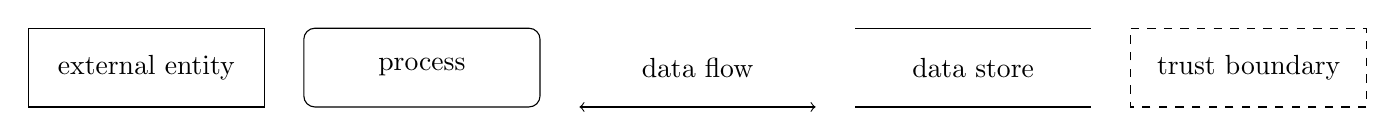
\begin{tikzpicture}
                                \begin{scope}[shift={(0, 0)}]
                                    \draw (0, 0) -- (3, 0) -- (3, -1) -- (0, -1) -- cycle;
                                    \node at (1.5, -0.5) {external entity};
                                \end{scope}
                                \begin{scope}[shift={(3.5, 0)}]
                                    \draw[rounded corners] (0, 0) -- (3, 0) -- (3, -1) -- (0, -1) -- cycle;
                                    \node at (1.5, -0.5) {process};
                                \end{scope}
                                \begin{scope}[shift={(7, 0)}]
                                    \draw (0, -1) edge[<->] (3, -1);
                                    \node at (1.5, -0.5) {data flow};
                                \end{scope}
                                \begin{scope}[shift={(10.5, 0)}]
                                    \draw (0, -1) -- (3, -1);
                                    \draw (0, 0) -- (3, 0);
                                    \node at (1.5, -0.5) {data store};
                                \end{scope}
                                \begin{scope}[shift={(14, 0)}]
                                    \draw[dashed] (0, 0) -- (3, 0) -- (3, -1) -- (0, -1) -- cycle;
                                    \node at (1.5, -0.5) {trust boundary};
                                \end{scope}
                            \end{tikzpicture}
                        \end{center}
                        For example, if two processes exist inside the same trust boundary, we generally don't need to be worried about attacks from one process to the other.
                        However, we do need to be concerned about any data flow arrows that cross the boundaries.
                    \item identify threats (STRIDE / attack trees)
                        \smallskip

                        For STRIDE, we ask what may go wrong in each element of a DFD;
                        \begin{itemize}
                            \itemsep0em
                            \item \textbf{s}poofing \hfill pretend to be something else
                            \item \textbf{t}ampering \hfill modifying without permission
                            \item \textbf{r}epudiation \hfill denying to have performed an action
                            \item \textbf{i}nformation disclosure \hfill revealing information without permission
                            \item \textbf{d}enial of service \hfill prevent system from providing a timely service
                            \item \textbf{e}levation of privilege \hfill achieve more than what is intended
                        \end{itemize}
                        Threats may belong to more than one of these categories, and threats should be document by writing risk-based security tests when possible.
                        \medskip

                        Another approach is to create an attack tree, where the root node represents the goal of the attack, or the target asset.
                        Children are the steps to achieve the goal, and the leaves are concrete attacks; by default, sibling nodes represent \textbf{sufficient} steps (only one needs to be satisfied), but special notation is used to represent \textbf{necessary steps} (where all need to be satisfied).
                        Note that the course uses lines between the arrows to denote necessary steps, however I will be using matching colours.
                        For example;
                        \begin{center}
                            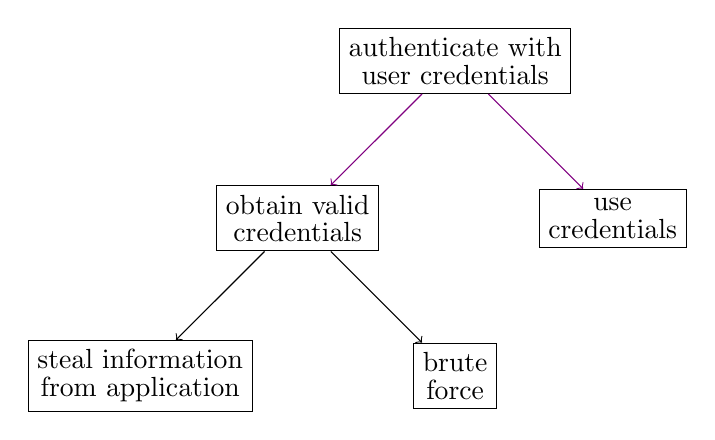
\begin{tikzpicture}[x=2cm, y=2cm];
                                \node[draw] (o) at (0, 0) {\shortstack{authenticate with\\user credentials}};
                                \node[draw] (ol) at (-1, -1) {\shortstack{obtain valid\\credentials}};
                                \node[draw] (or) at (1, -1) {\shortstack{use\\credentials}};
                                \node[draw] (oll) at (-2, -2) {\shortstack{steal information\\from application}};
                                \node[draw] (olr) at (0, -2) {\shortstack{brute\\force}};
                                \draw
                                (o) edge[->, violet] (ol)
                                (o) edge[->, violet] (or)
                                (ol) edge[->] (oll)
                                (ol) edge[->] (olr);
                            \end{tikzpicture}
                        \end{center}
                        This can also be represented in a textual format, where the root is a bullet point, and the necessary steps are `+', with the sufficient points being `-'.
                        \medskip

                        Attack trees are an alternative to STRIDE, for each element in a DFD, if the goal of an attack tree is relevant, the tree can be traversed to identify possible attacks.
                        Similarly, we can look at previously seen attack trees.
                        \medskip

                        It's important to focus on realistic threats.
                        The threats that should be considered depend on the system being modelled, the budget, and the value of what is being protected.
                    \item evaluate and address threads (DREAD / META)
                        \smallskip

                        The two main approaches for evaluating threats are qualitative (based on insight, experience, and expectations) and quantitative (based on some numerical score).
                        However, quantifying risk is difficult (and realistic parameters are hard to estimate), rare events are also hard to predict (and therefore hard to quantify).
                        \medskip

                        The DREAD methodology is a ranking from 5 to 15, developed by Microsoft;
                        \begin{center}
                            \begin{tabularx}{\textwidth}{|cl|X|X|X|}
                                \hline
                                & rating & high (3) & medium (2) & low (1) \\
                                \hline
                                \textbf{D} & damage potential & attacker can subvert full security system, get full trust authorisation, run as administrator, upload content & leaking sensitive information & leaking trivial information \\
                                \textbf{R} & reproducibility & attack can be reproduced every time and does not require a timing window & attack can be reproduced but only with a timing window and particular race situation & attack is difficult to reproduce, even with knowledge \\
                                \textbf{E} & exploitability & novice programmer could make the attack in a short time & skilled programmer could make the attack & extremely skilled person and in-depth knowledge to exploit every time \\
                                \textbf{A} & affected users & all users, default configuration, key customers & some users, non-default configuration & very small percentage of users, obscure feature \\
                                \textbf{D} & discoverability & published information explains the attack, vulnerability in most commonly used feature and is noticeable & vulnerability in seldom-used part of product, would take thinking to see malicious use & obscure bug, and users unlikely to work out damage potential \\
                                \hline
                            \end{tabularx}
                        \end{center}
                        After a thread is addressed, a response should be recommended;
                        \begin{itemize}
                            \itemsep0em
                            \item \textbf{m}itigate \hfill make threat harder to exploit
                                \smallskip

                                For example, if the threat was password brute-forcing, mitigations could require better passwords or locking accounts after some number of failed attempts.
                            \item \textbf{e}liminate \hfill remove feature exposed to threat
                            \item \textbf{t}ransfer \hfill let another party assume the risk
                                \smallskip

                                Continuing with the login scenario, we can use a third party login system.
                                The cost is that the third party has information about customers, and that legal responsibility may still remain (despite technological risk being transferred)
                            \item \textbf{a}ccept \hfill when other options are impossible or impractical
                                \smallskip

                                If someone was to guess the password on the first try, nothing can prevent it.
                                It's important to keep track that the threat remains active.
                        \end{itemize}
                        Responses should be documented, such as in a project issue tracker.
                \end{enumerate}
        \subsection*{Week 2}
            \subsubsection*{Authentication}
                The main application of computer passwords are the protection of cryptographic keys or user authentication.
                Password based authentication is widely used as it is easy to understand, easy to implement, and deploy.
                Some implementations are as follows;
                \begin{itemize}
                    \itemsep0em
                    \item \textbf{plain-text passwords}
                        \begin{enumerate}[1.]
                            \itemsep0em
                            \item store all credentials in a file (~/etc/passwd~ or ~/etc/shadow~);
                                \begin{lstlisting}
                                    alice:foo
                                      bob:bar
                                \end{lstlisting}
                            \item user gives username and password
                            \item check if username is present, if it is; check password matches stored
                            \item grant / deny access
                        \end{enumerate}
                        This becomes a valuable target for hackers, as this file alone allows for anyone with the file to impersonate users on the system.
                    \item \textbf{encrypted passwords}
                        \smallskip

                        This implementation uses \textbf{symmetric encryption}, where the encryption and decryption are done with the same key.
                        The steps are similar to above, however \textbf{encrypted} passwords are stored in the file - the remaining steps are the same (except step 3, where we check if the decrypted version of the stored password matches the given password).
                        \medskip

                        This is more secure than before; where the attack tree now has two children (need to obtain the encrypted file \textbf{and} the decryption key).
                    \item \textbf{password hashes}
                        \smallskip

                        In contrast to before, this uses a \textbf{one-way} hashing function, which should not be reversed.
                        Similar to before, we now store \textbf{hashed} passwords in the file.
                        Step 3 now applies the hash function to the presented password, checking that it matches the hash stored in the file.
                        While this is more secure than the previous, it's susceptible to an \textbf{offline dictionary attack}, where a large table of candidate passwords and corresponding hashes are built up.
                        A hash in the stolen password file can now be looked up in the \textbf{rainbow table}.
                    \item \textbf{salted hashes}
                        \smallskip

                        A \textbf{salt} is a cryptographically random string, which is combined with the password in the hash.
                        The salted hashes are stored in the file, in the format ~username:salt:salted\_hashed\_password~ (where the salt is specific to the user);
                        \begin{lstlisting}
                            alice:61C82:2CFAD1C96B8236072823B77EDBF150B1
                              bob:8B4D8:7FBA1AFAAB57793255B59A8D596449D3
                        \end{lstlisting}
                        Step 3 now combines the given password with the salt, hashes it, and checks it against the salted and hashed password in the file.
                        The remaining steps are the same.
                        \medskip

                        It's now impractical to build a rainbow table, as a different dictionary will be needed for each possible salt.
                \end{itemize}
                The Linux password file stores passwords in the following format;
                \begin{center}
                    ~username:password\_data:parameters~
                \end{center}
                Where the ~password\_data~ is stored in the following format;
                \begin{center}
                    ~\$hash\_function\_id\$salt\$password~
                    \smallskip

                    \begin{tabular}{l|l}
                        ~hash\_function\_id~ & algorithm \\
                        \hline
                        ~1~ & ~md5~ \\
                        ~2a~, ~2y~ & ~blowfish~ \\
                        ~5~ & ~sha256~ \\
                        ~6~ & ~sha512~
                    \end{tabular}
                \end{center}
                The problem with passwords is usability; complex passwords are a burden to users.
                Security questions are also dangerous, as common answers can quite easily be found online via social media.
                Hints also tend to be chosen such that they easily give away the password.
                Ideally, we choose a password we can't remember, and don't write it down.
                However, it's hard for humans to choose and remember good passwords, therefore users tend to use memorable passwords (and users with common interests may use similar passwords).
                \medskip

                Because of this, offline dictionary attacks don't need to try every possible passwords; they can start with a dictionary of common words, and then apply rules to generate variants.
                This can include `leetspeak', where letters are substituted with similar looking numbers, using a few uppercase letters, and appending common years.
                \medskip

                Another issue is password reuse, leading to \textbf{online dictionary attacks}.
                In this situation, attackers submit login combinations to a live authentication system (rather than a stolen password file).
                Usernames are quite easy to find (as they are public) or can just be email addresses.
                Previously used passwords are easily to find, where lists of passwords from hacked websites can easily be found.
                \medskip

                Defences against this can include limiting the number of attempts per username / IP before blocking access.
                Another approach is to use CAPTCHAs, preventing simple automation attacks (however it can inconvenience legitimate users).
                Honeypot accounts can also be made, which are easily cracked.
                Requests can be blocked from a device attempting to login to one of these accounts.
                \medskip

                The best practices to build passwords are as follows;
                \begin{itemize}
                    \itemsep0em
                    \item filters to select, random looking passwords (force user to use good passwords)
                    \item hash passwords with functions like ~PBKDF2~ (password based key derivation function) or ~bcrypt~ (which take long enough to prevent hackers from building rainbow tables)
                    \item don't force users to change passwords often (otherwise users will choose easy passwords)
                    \item don't fail with ``user not found''; this allows attackers to find valid users
                    \item block account or requests from same IP after too many attempts
                    \item on a successful long, show information about last login (allows user to report suspicious logins) and notify user if login is from a different machine / location
                \end{itemize}
                On the other hand, some practices that could be followed by users (to enhance passwords);
                \begin{itemize}
                    \itemsep0em
                    \item \textbf{password managers}
                        \smallskip

                        Password managers allow users to handle strong passwords for many different websites, as well as avoid phishing sites.
                        However, they are a single point of failure; if the master password is lost, all the other accounts are lost, similarly if a hacker obtains the master password, all passwords are obtained.
                        Online managers are exposed to hackers, whereas offline managers can potentially be unavailable.
                    \item \textbf{2FA} (2$^\text{nd}$ factor authentication)
                        \smallskip

                        2FA prevents attacks based on weak / stolen passwords.
                        However, the main downsides include being locked out of an account without the device, as well as users being given a false sense of security (leading to weaker passwords).
                        It also introduce another device into the user's \textbf{Trusted Computing Base}.
                    \item \textbf{OAuth or Single Sign On}
                        \smallskip

                        This allows for authentication via a trusted identity provider, such as some social networks, delegating responsibility to a third party.
                        However, this does lead to the cost of giving a third party your user data.
                \end{itemize}
                There are also alternatives to passwords entirely, including;
                \begin{itemize}
                    \itemsep0em
                    \item \textbf{hardware tokens}
                        \smallskip

                        Commonly used by banks (creating single use passwords / tokens for logins or transactions).
                        These are expensive and hard to replace.
                    \item \textbf{biometric authentication}
                        \smallskip

                        It's impossible to replace if ``lost'' or revealed (spoofed).
                    \item \textbf{RFID tags}
                        \smallskip

                        As a physical object, they are at risk of theft or misplacement.
                        Similarly, due to the nature of RFID, it can be susceptible to proximity based attacks.
                    \item \textbf{passwordless authentication}
                        \smallskip

                        A lower value website can be authenticated by the user proving they have access to a certain email.
                        When the user wishes to login, a temporary pin is generated and sent to a given email.
                \end{itemize}
            \subsubsection*{Pentesting}
                \textbf{Penetration testing} is the process of paying someone to break into a system or organisation, and report the weaknesses (can also include physical security of the building).
                It's important to scope the pentesting, particularly the goals we are trying to achieve (what's being accessed).
                Once this is agreed, restrictions on the targets, tools, techniques, and side effects (cannot wipe out an entire database to prove it is vulnerable) need to be discussed.
                \medskip

                A pentesting exercise is also defined by the amount of available information;
                \begin{itemize}
                    \itemsep0em
                    \item \textbf{black box} \hfill no information, all has to be discovered from a given high-level goal
                    \item \textbf{grey box} \hfill selected information, e.g; there is an intranet, which contains a database server
                    \item \textbf{white box} \hfill extensive information about the system, possibly including source code
                \end{itemize}
                It's hard to ensure a pentester has tried ``hard enough'', and one option is to have several teams playing against each other.
                Certifications (such as \textit{CISSP}) commend higher fees.
                \medskip

                PTES (Penetration Testing Execution Standard) are a set of fundamental principles and technical guidelines for pentesting, with the following key steps;
                \begin{enumerate}[1.]
                    \itemsep0em
                    \item pre-engagement interactions \hfill sign contract, define scope
                    \item \textbf{intelligence gathering}
                        \smallskip

                        This can be split into two phases;
                        \begin{itemize}
                            \itemsep0em
                            \item \textbf{passive} information gathering
                                \smallskip

                                The aim is to build as much information about the target system without engaging with the target itself.
                                We want to have enough information to build a data-flow diagram of the target, in order to drive the next phase, as well as information about the network structure of the target.
                                However, we don't want to reveal our presence at this phase, and one technique is to prevent any connection to the target (by blocking access through a firewall or proxy).
                                \medskip

                                One approach is to look for information made public, including possible blog posts from the company which may contain relevant information.
                                From there, we can find any web presence - looking at source code for any links, form fields, as well as references to open source code used (possibly finding bugs or hardcoded credentials) and protocols.
                                While accessing the website should be fine, it's also possible to hide any presence at this point by looking at cached versions of the site only.
                                It's important to note that even publicly accessible data may be protected by law.
                                \smallskip

                                One technique that can be used is \textbf{Google Hacking}, which uses search engine operators to locate sites;
                                \begin{itemize}
                                    \itemsep0em
                                    \item ~ext:pdf~ \hfill search with specific extensions
                                    \item ~site:example.com~ \hfill search within a given website only
                                    \item ~"index.html" inurl: -html~
                                        \smallskip

                                        find inside page, but without ~html~ in the URL (find exposed directories)
                                    \item ~allintext:"Powered by phpbb"~ \hfill locate sites running known vulnerable software
                                \end{itemize}
                            \item \textbf{active} information gathering
                                \smallskip

                                We can collect more in-depth information if we are willing to contact our directly, at the risk of being detected (therefore it is better to do it from a different IP than the one used for exploitation).
                                To verify gathered email addresses, emails could be sent to these addresses and checked for any bounces.
                                Network probing can also be done, identifying what subnet addresses are active and what ports accept communications.
                                It's also possible to identify services, by performing \textbf{banner grabbing} as some services send identifying information by default, or by reverse-engineering the protocol.
                                It may be sufficient to send random data and to observe the error message.
                        \end{itemize}
                    \item \textbf{threat modelling}
                    \item \textbf{vulnerability analysis}
                        \smallskip

                        The target may not be fully patched.
                        From there, we can look in the CVE database for any vulnerabilities in the previously identified components.
                        Automated tools can be used to systematically scan the target (however this generates a large amount of traffic).
                        \medskip

                        However, if the system is patched, we can attempt to look for new vulnerabilities.
                        If the source code is available, we can use static analysis tools or perform this by hand (which can be very slow).
                        Another approach is to trigger vulnerabilities with educated guesses like SQLi or XSS.
                        \medskip

                        Another approach is to find credentials, by either looking for default logins or finding password hashes published by hackers.
                    \item \textbf{exploitation}
                        \smallskip

                        In this phase, we actually act on the vulnerabilities identified before.
                        For example; if we have collected credentials, we can attempt to use them to see if they work.
                        We can also run publicly available exploits, either manually (and with our own exploits), or using automated tools such as \textit{Metasploit} (tailored to verified vulnerabilities only, not just everything the tool can do).
                    \item \textbf{post-exploitation}
                        \smallskip

                        If the exploited account isn't an administrator, privilege escalation should be attempted.
                        Typical goals to prove access include;
                        \begin{itemize}
                            \itemsep0em
                            \item steal data
                            \item send data back to the hacker
                            \item maintain access
                            \item manipulate logs to cover tracks
                            \item pivot; use host to exploit other targets on LAN
                        \end{itemize}
                    \item reporting
                \end{enumerate}
            \subsubsection*{Networks Background}
                Most of this should be covered in the \textbf{CO212} module last year.
            \subsubsection*{LAN Security}
                We want to clarify the principles of what we consider as legitimate users and attackers on the networks, and the capabilities;
                \begin{itemize}
                    \itemsep0em
                    \item \textbf{participant}
                        \smallskip

                        A participant can send and receive legitimate packets that respect the protocol (for example web browsers and web applications).
                    \item \textbf{eavesdropper}
                        \smallskip

                        On the other hand, an eavesdropper can read packets sent to others, and will not / cannot participate.
                        Examples of eavesdroppers include wiretappers and sniffers on a broadcast network.
                    \item \textbf{off-path}
                        \smallskip

                        In contrast, an off-path attacker is connected to the same network between the client and the server, however is not in the same local area network (and cannot sniff packets).
                        However, it can participate and create arbitrary packets (which may not abide by the protocols).
                        Examples of this include independent machines connected to the same WiFi.
                    \item \textbf{MITM (man in the middle)}
                        \smallskip

                        These are more powerful and completely control the link between one host and the rest of the network.
                        They can participate like a regular participant, but can also read, modify, or delete packets.
                        Examples of this include a proxy, an ISP, a router, or WiFi access point (therefore we should be careful on untrusted networks).
                \end{itemize}
                \begin{center}
                    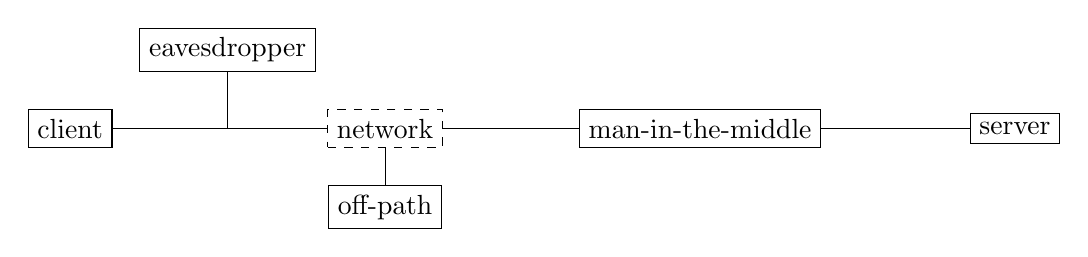
\begin{tikzpicture}
                        \node[draw, dashed] (n) at (1, 0) {network};
                        \node[draw] (c) at (-3, 0) {client};
                        \node[draw] (mitm) at (5, 0) {man-in-the-middle};
                        \node[draw] (s) at (9, 0) {server};
                        \node[draw] (op) at (1, -1) {off-path};
                        \node[draw] (e) at (-1, 1) {eavesdropper};

                        \draw
                        (c) -- (n)
                        (n) -- (mitm)
                        (mitm) -- (s)
                        (op) -- (n)
                        (e) -- (-1, 0);
                    \end{tikzpicture}
                \end{center}
                Within the same LAN, devices send messages to each other based on MAC (Media Access Control) addresses.
                The DHCP (Dynamic Host Configuration Protocol) tells new hosts their IP addresses (and other configuration information).
                ARP (Address Resolution Protocol) is used to find the MAC of an IP on the same LAN.
                \medskip

                As a device typically communicates by asking for data to be sent to a device with a given MAC, LANs typically rely on broadcast medium such as cable (Ethernet) or wireless (WiFi).
                Conflict resolution requires a minimum packet size, and if this padding data is not properly initialised (either with zeroes or dummy data) - and contains more bytes from the buffer, this may lead to data disclosure.
                Eavesdroppers hosts can also sniff the network (and we should assume that hosts connected to the network can see whatever we send).
                \medskip

                Assume a switch with 3 ports, and devices $A$, $B$, and $C$ connected to ports 1, 2, and 3 respectively, where $C$ is the attacker.
                \textbf{MAC flooding} is done in two phases, to force the switch to broadcast traffic;
                \begin{enumerate}[1.]
                    \itemsep0em
                    \item The attacker floods the CAM table with frames with invalid source MACs ($X \to ?$, $Y \to ?$, etc), preventing valid hosts from creating CAM entries.
                    \item A message $A \to B$ is now flooded out to both $B$ and $C$, since no CAM entries exist for the valid hosts.
                \end{enumerate}
                Countermeasures to this include limiting the number of MAC addresses from a single port as well as keeping track of authorised MAC addresses in the system.
                \medskip

                Another attack is \textbf{ARP poisoning}.
                By design, MAC is easy to spoof (as a way to deal with conflicting hardware).
                An attacker can change its MAC address in order to evade access control mechanisms.
                An off-path attacker spoofing the router can become a MITM.
                The process for poisoning is as follows;
                \begin{enumerate}[1.]
                    \itemsep0em
                    \item switch needs to find MAC corresponding to an IP
                    \item attacker spoofs MAC of victim and replies like the victim
                    \item message is forwarded to both ports that replied (victim and attacker)
                \end{enumerate}
                Countermeasures include static ARP rules (which can be inconvenient), or to detect spoofed ARP messages (at which point both hosts are kicked off, and an administrator is likely notified).
        \subsection*{Week 3}
            \subsubsection*{IP Security}
                The IP (Internet Protocol) is a best effort (may drop / reorder packets) protocol which delivers packets between \textbf{source} and \textbf{destination} hosts.
                IP addresses are structured in a hierarchical way and guides routing.
                However, since these may travel across networks with smaller packet sizes, IP packets can be fragmented.
                The \textbf{D}on't \textbf{F}ragment, \textbf{M}ore \textbf{F}ragments flags indicate the type, the fragment offset field gives the \textbf{position} of the fragment in the \textbf{original} fragment, and \textbf{identification} differentiates fragments for different packets.
                Different operating systems treat duplicate IP fragments in different ways - this can be used for OS fingerprinting.
                The TTL (time to live) field is used to discard packets that take too many steps to reach a destination; when the TTL is decremented (at each hop) to zero, the packet is discarded and an ICMP error message is sent to the source.
                \medskip

                TTL is used to prevent loops in networks (zombie packets).
                However, it can also be used by the \textbf{Traceroute} algorithm to identify devices on the path to a target.
                By sending packets with an incrementing TTL (first 1, then 2, and so on), each ICMP error message should come from a host on the path to the destination.
                This can be used to gather information about a target network (such as firewalls).
                \medskip

                The source IP can be easy to spoof (as it is not authenticated).
                An off-path attacker can send packets with a target IP as the source, leading to the target receiving responses.
                This is used for attacks such as amplification based DDoS or idle scanning.
                \medskip

                The Internet, by design, is a decentralised network of untrusted networks.
                As such, packets travel through untrusted hosts, hence MITM attackers (such as an ISP) could directly read packets and modify payloads.
                BGP routing is partly based on trust.
                As a single AS (autonomous system) cannot track all IP addresses, they must ask each other for a route to reach an IP of a distant AS.
                They may misbehave (BGP hijacking) by advertising false routes, diverting this traffic, and perform MITM attacks.
                \medskip

                There is an ongoing global effort to secure BGP; \textbf{MANRS (Mutually Agreed Norms for Routing Security)}, supported by the Internet Society and big players.
                This specifies best practices for network operators (ISPs), Internet exchange providers (IXPs), content delivery networks, and cloud providers.
                The \textbf{RPKI (Resource Public Key Infrastructure)} is the idea to use public key infrastructure to propagate trust down the address hierarchy.
                When an AS is looking for a route to reach a system, it will be prevented with BGP advertised routes (as well as certificates, which can only be provided by the owner, or a correct path).
                \medskip

                IPsec adds security to IP with two main protocols, in two modes (transport and tunnel, where the former protects the IP payload only, and the latter \textbf{also} protects the IP header);
                \begin{itemize}
                    \itemsep0em
                    \item \textbf{authentication header (AH)}
                        \smallskip

                        Preserve packet integrity (recipient will know if tampered with) and protect authentication (recipient will be confident about who the sender is).
                        Packet inspection is allowed, and isn't blocked by firewalls.
                    \item \textbf{encapsulating security payload (ESP)}
                        \smallskip

                        This preserves confidentiality of the payload, but may be blocked by security.
                \end{itemize}
                ESP tunnel mode is commonly used to implement VPNs.
                This gives network layer confidentiality, source authentication, data integrity, and replay-attack prevention.
                In this mode, the protocol is changed from ~proto=TCP~ in the original IPv4 datagram to ~proto=ESP~.
                After the destination IP address, the original TCP header and payload is replaced with the following;
                \begin{itemize}
                    \itemsep0em
                    \item SPI (security parameters index)
                    \item sequence header
                    \item IP header
                    \item TCP header + payload
                    \item padding (variable), padding length, and next IP
                    \item (optional) authentication data
                \end{itemize}
                The lecture then goes over IPv6 (see \textbf{CO212}); we focus mostly on IPv4 in this course.
                \medskip

                TCP (more detail in \textbf{CO212}) has security issues stemming from an easily accessible state.
                The sequence numbers are easily predictable, as they are the previous number added with the bytes exchanged;
                \begin{itemize}
                    \itemsep0em
                    \item a MITM attacker could read the current sequence number and inject new packets (TCP session hijacking)
                    \item an off-path attacker could try to guess the correct sequence number (blind spoofing, read \textit{Off-Path Hacking})
                \end{itemize}
                Typical countermeasures include introducing a time-delay and discarding race-condition packets, or use IDS or protect the payload (e.g. HTTPS).
                \medskip

                Port scanning may be a crime (when unauthorised), depending on the legal jurisdiction.
                The idea is to use the initial steps of the protocol to determine whether a port is open;
                \begin{itemize}
                    \itemsep0em
                    \item TCP ~connect()~
                        \smallskip

                        If the HTTP port is open, sending ~SYN + Port 80~ to a host will result in a response of ~SYN/ACK~.
                        We can then send ~ACK~ and ~RST~ to close the connection.
                        However, if a port was closed (say FTP), sending ~SYN + Port 21~ to a host will result in a response of ~RST~.
                    \item TCP idle scan
                        \smallskip

                        To do this, we perform the following steps;
                        \begin{enumerate}[1.]
                            \itemsep0em
                            \item find an idle host (one that is online, but not used actively, such as a printer during the night)
                            \item check available IPID on printer by sending ~SYN/ACK~ to printer, will respond with ~RST,IPID=x~
                            \item send ~SYN,src=<idle host>~ to the target (pretend to be target host)
                            \item if the port is closed, will reply with ~RST~ to the printer, or ~SYN/ACK~ if open
                            \item if the port was open (~SYN/ACK~), the idle host will reply to the target with ~RST,IPID=x+1~
                            \item perform step 2 again; if we get ~RST,IPID=x+1~, we know the port was closed on the target, however if we get ~RST,IPID=x+2~, we know it is open.
                        \end{enumerate}
                        This can evade some port scanning protection which only monitors connections between internal and external hosts, and not monitoring at an internal level.
                \end{itemize}
                UDP is connectionless, which has low overhead and low latency.
                This can be used for broadcasting or multicasting packets.
                There is no guarantee that the data reaches the destination, and there is no integrity (optional checksum) - it is up to the application layer to make sense of a UDP stream.
                See \textbf{CO212} for more details.
                \medskip

                UDP scans are harder, as we do not expect any acknowledgements (compared to TCP).
                We can send a generic UDP header with no payload to target ports; if we get a UDP response, the port is open, otherwise if we receive an ICMP error the port is closed (or filtered by a firewall).
                However, if we timeout without a response, the port may be open (but hosting a service that drops ill-formed packets), or the port may be filtered by a firewall.
                If we encounter this case, we can probe the port again using UDP packets, but with payloads specific to a protocol (e.g. DNS query).
                This adds to the difficulty; it is more time consuming (due to a lack of response) and may take multiple attempts to resolve ports.
                In addition, they are less precise, as some protocols just cannot be probed.
                \medskip

                The key threats of TCP/IP are as follows;
                \begin{itemize}
                    \itemsep0em
                    \item \textbf{host and port scanning}
                        \smallskip

                        Used by hackers during active information gathering, with request being hidden within normal network traffic.
                    \item \textbf{port sweep}
                        \smallskip

                        Attacker looks for specific service on many machines (likely looking for a vulnerable service).
                        Nowadays, if we encounter a port sweep, it's possible it's a security researcher trying to find the number of accessible webcams (or some sort of insecure IoT device).
                    \item \textbf{malicious traffic}
                        \smallskip

                        Normal connection, but may send malicious data that exploits the implementation of the networking stack.
                    \item \textbf{(D)DoS}
                        \smallskip

                        Flood target with high volume of network traffic (commonly done with botnets).
                        This either fully takes the target down, degrades performance, or increases costs.
                \end{itemize}
                Port knocking is a technique to hide a service form port sanning (either by a system administrator, or an attacker attempting to hide a backdoor);
                \begin{enumerate}[1.]
                    \itemsep0em
                    \item sequential / random scan only finds closed ports
                    \item client shares a secret with sever, identifying specific ports to probe in a fixed order (e.g. 3,1,2,4) - the last probe is replied to by the server with a random port $n$, where the service is located
                    \item client connects to service on port $n$
                \end{enumerate}
            \subsubsection*{Network Defences}
                Here we take a high level overview of classic network defence systems (mainly firewalls and IDSs (intrusion detection systems)).
                \medskip

                The main firewall protects all internet traffic.
                The internal network is kept separate from Internet-facing services (in the demilitarised zone) such as a web server or FTP server.
                In the internal network, we may have private databases or sensitive machines; generally data we don't want to share with the outside.
                \medskip

                The main goal of a firewall is to enforce security policies on all inbound / outbound traffic for the subnetwork it is trying to protect.
                A firewall will typically specify what hosts can communicate with what over hosts (and what protocols, or how much data can be exchanged - general properties of traffic).
                This not only can protect against attacks, but can also control what can be done by hosts.
                It's common to have a centralised firewall to ensure consistent policies achieving the same goal.
                Once the general network-wide policies are enforced, there may be other dedicated firewalls for subnets (with modern hosts also having local firewalls).
                Firewalls can be either;
                \begin{itemize}
                    \itemsep0em
                    \item dedicated network appliances (with purpose built hardware) \hfill \textit{Cisco}, \textit{CheckPoint}
                    \item kernel-level applications (general purpose hosts) \hfill ~iptables~, ~pf~, Windows firewall
                \end{itemize}
                They are valuable targets for attackers (if it can be owned, it runs at a privileged position on the victim network / OS).
                \medskip

                Policies can be either of the following;
                \begin{itemize}
                    \itemsep0em
                    \item \textbf{packet filters} \hfill decision based on individual packet
                        \smallskip

                        This can take into account protocol header fields, source / destination addresses, and ports.
                    \item \textbf{stateful filters} \hfill take state into account
                        \smallskip

                        Keep track of sessions (for TCP) and check if the packet is part of an established connection.
                        It can also look at timeouts, and the amount of bandwidth used.
                    \item \textbf{both} \hfill combination, and also support payload inspection
                \end{itemize}
                Intrusion detection systems are more powerful than firewalls, and allow for deep packet inspection.
                This allows for decisions to be made based on the payload (not just headers), and raise an alert (IDS) or drop packets (IPS - intrusion prevention system).
                They aim to detect or prevent attacks, such as active information gathering (including scans or sweeps), DDoS, worms (as they have a global view of the network), and application layer attacks.
                The approaches are typically divided into the following;
                \begin{itemize}
                    \itemsep0em
                    \item \textbf{signature based}
                        \smallskip

                        Most common case.
                        They have rules to detect packets that have been observed in the past to be part of / have characteristics of a known attack.
                        Generalising rules (to catch variants) can cause false positives; there is a trade-off between sensitivity and specificity.
                        These are typically human generated.
                        A \textit{ModSecurity} example for detecting XSS is as follows;
                        \begin{lstlisting}
                            SecRule ARGS|REQUEST_HEADERS "@rx <script>"
                            id:101,msg:'XSS Attack',severity:ERROR,deny,status:404
                        \end{lstlisting}
                        This applies the rule to the arguments or the headers, looking for a regex that contains the script tag, and denies the request with a 404.
                        They are good for matching attacks with known patterns, however they cannot catch unseen attacks.
                        Once a signature is known to be known, it can be easy to bypass (similar to antivirus).
                        They focus on content rather than intent, and are better for stopping automated attacks than manual ones.
                        \medskip

                        Each rule is simple, however applying the rules to each packet becomes more expensive with more rules and packets.
                        This can be evaded with IP fragmentation.
                        Here we assume there are 10 hops from an attacker to the monitor, and a further 8 hops to the victim (18 hops in total);
                        \begin{enumerate}[1.]
                            \itemsep0em
                            \item fragment a suspicious IP packet in 2 (~ttl=20,seq=6...9: USER~ and ~ttl=20,seq=10...3: root~)
                            \item traceroute to determine distance to IDS and target
                            \item send fragment 1 (~ttl=20,seq=6...9: USER~) to reach the target
                            \item send a replacement of fragment 2 (~ttl=12,seq=10...3: root~)  so that the IDS sees it, but the target does not; note that the TTL is 12, which clears the monitor but expires before the victim
                            \item IDS now decides that the communication is safe (it sees ~USER|nice~)
                            \item send malicious fragment 2 (~ttl=20,seq=10...3: root~), which reaches the target, the target now has ~USER|root~
                            \item IDS does not interpret the message sent in step 6 as related to the one sent in step 3
                        \end{enumerate}
                    \item \textbf{anomaly detection based}
                        \smallskip

                        This attempts to generalise to attacks that haven't been previously seen.
                        The idea is to learn what normal traffic looks like, and point out statistical anomalies based on features such as the protocol used, packet size, time, order, hosts, etc.
                        It learns a model of benign traffic, with heterogeneous features, either categorical (TCP/UDP/...), or continuous (such as size).
                        It can detect unseen attacks, where there is no existing signature, however it can suffer from false positives (where we have uncommon traffic).
                        \medskip

                        Simple examples could be packets which are too large, or accesses to high numbered ports which are not typically used (which are typically used as source ports) - these are \textbf{point} anomalies, which is one sample being anomalous with respect to others.
                        On the other hand, \textbf{contextual} anomalies are only anomalous in specific contexts, but not in others.
                        For example, high bandwidth usage may be an anomaly at night but not during the day.
                        Furthermore, there are \textbf{collective} anomalies, which are anomalous with respect to all available samples; for example, a TCP connect scan to the same port of many hosts could be detected as port sweep.
                        \medskip

                        Models used typically are statistical (non-parametric for histograms or PCA), or parametric (regression), or are classification based (Bayesian networks, neural networks, SMVs, or random forests).
                        Training is commonly semi-supervised, with an unlabelled dataset consisting of only normal events.
                        An unsupervised training mode is unlabelled data possibly containing some anomalies, and a supervised training contains labels for both normal and anomalous events.
                     \item \textbf{specification based}
                        \smallskip

                        Logical rules / simple languages dictate whether a packet should be accepted or rejected.
                        However, it's hard to define rules, avoid conflicts, and may be inconsistent.
                \end{itemize}
            \subsubsection*{DNS (Domain Name System)}
                The DNS allows us to identify hosts via easy to remember, descriptive hostnames, rather than IP addresses.
                This separates the logical address of a service from the physical address of the host (which allows for hostnames to stay the same when network providers are switched).
                We need to know the IP address of the target hostname, which can be obtained by a local DNS client / resolver in DNS resolution.
                Once a name is cached, it will be valid for a limit amount of time.
                If a name is in the cache, we can use that, otherwise the resolver queries an external primary / recursive DNS server.
                Typically, they are short queries and responses, fitting into a single UDP packet (512 bytes) - if more data needs to be exchanged, it falls back to TCP.
                Domain names are organised in a hierarchical manner, DNS is managed by ICANN/IANA, who also run the root DNS servers (note that ~com~ is a gTLD, and ~uk~ is a ccTLD (country));
                \begin{center}
                    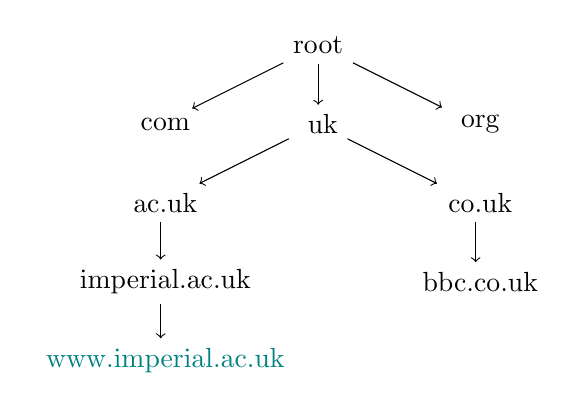
\begin{tikzpicture}[x=2cm]
                        \node (o) at (0, 0) {root};
                        \node (ol) at (-1, -1) {~com~};
                        \node (oc) at (0, -1) {~uk~};
                        \node (or) at (1, -1) {~org~};
                        \node (ocl) at (-1, -2) {~ac.uk~};
                        \node (ocr) at (1, -2) {~co.uk~};
                        \node (oclc) at (-1, -3) {~imperial.ac.uk~};
                        \node (ocrc) at (1, -3) {~bbc.co.uk~};
                        \node[teal] (oclcc) at (-1, -4) {~www.imperial.ac.uk~};
                        \draw
                        (o) edge[->] (ol)
                        (o) edge[->] (oc)
                        (o) edge[->] (or)
                        (oc) edge[->] (ocl)
                        (oc) edge[->] (ocr)
                        (ocl) edge[->] (oclc)
                        (ocr) edge[->] (ocrc)
                        (oclc) edge[->] (oclcc);
                    \end{tikzpicture}
                \end{center}
                A domain name which can be used to fully access a host is called a fully-qualified domain name (\teal{FQDN}).
                The process of DNS resolution, when the local cache doesn't have it stored is as follows;
                \begin{enumerate}[1.]
                    \itemsep0em
                    \item user asks primary DNS server for IP address of ~example.com~
                    \item primary DNS server asks root server for \textbf{location of} IP address of ~example.com~
                    \item root server tells primary DNS server to ask ~.com~ namespace
                    \item primary DNS server asks ~.com~ namespace for IP address of ~example.com~
                    \item namespace tells primary DNS server to check primary DNS server of ~example.com~
                    \item primary DNS server asks primary DNS server of ~example.com~ the IP address of ~example.com~
                    \item primary DNS server of ~example.com~ tells user's primary DNS server the IP address of ~example.com~
                    \item user's primary DNS server tells user IP address of ~example.com~
                \end{enumerate}
                Common DNS records include;
                \begin{center}
                    \begin{tabularx}{\textwidth}{lX}
                        resource record & description \\
                        \hline
                        ~A~ & mapping of a name to address (IPv4) - performs primary function of DNS; converting names to addresses \\
                        ~AAAA~ & same as ~A~, but for IPv6 \\
                        ~NS~ & resolver doesn't know, instead replies with a name server which knows (identifies DNS server function as authority of the zone, each DNS server must be represented by a NS record, whether primary, master, or secondary) \\
                        ~SOA~ & identifies which server is the primary one (start of authority); each zone must have an SOA record and only one SOA record can be in a zone \\
                        ~PTR~ & (pointer) does reverse of ~A~; provides a mapping from address to name \\
                        ~CNAME~ & creates an alias that points to canonical name (real name) of a host identified by an ~A~ record - can be used to check cache for the real name \\
                        ~MX~ & identifies a system that will direct email traffic (mail exchange) \\
                        ~NXDOMAIN~ & the name cannot be resolved, it is a non-existent domain (not registered or invalid)
                    \end{tabularx}
                    \vspace{-\baselineskip}
                \end{center}
                This structure leaves space for a MITM attack, recently done by the Turkish government in March 2014 (to block \textit{Twitter} access) by forcing ISPs to respond to DNS queries for ~twitter.com~ with the IP of a government website.
                \textit{DNSpionage} in 2019 had malicious actors compromise DNS resolution of key infrastructure, to spy on emails of certain individuals.
                Techniques included compromising DNS provider's admin panels (by simple brute force), changing the ~A~ records of target mail servers.
                Other cases involved hacking the TLD and changing the NS record to a rogue NS (providing legitimate address normally, but giving a malicious one for ~MX~ records).
                This lead to queries for target mail servers coming from victim IPs to a rogue mail server, and legitimate answers for other queries.
                \medskip

                Similar to TCP, DNS requests and responses are not authenticated.
                Attackers can map trusted domain names to malicious IP trivially with MITM (even some ISPs replace ~NXDOMAIN~ with adverts).
                Off-path attackers on LAN may be able to inject spoofed DHCP packets and advertise a malicious DNS resolver, or inject spoofed replies to DNS queries (after seeing the query ID).
                Routers can also be compromised to advertise malicious resolvers (\textit{DNSChanger} malware).
                DNS cache poisoning is when spoofed responses are being kept by intermediaries, giving a window of time.
                Name servers can also be hacked.
                \medskip

                DNSSEC protects the authenticity and integrity of DNS records with zones that have public / private keys.
                This forms a chain of trust; starting with the DNS root (the resolvers know public keys of root nodes).
                The parent nodes then use private keys to sign hashes of the child's public keys, allowing resolvers to check the authenticity of a node's public key.
                DNS resolution nodes then sign zone data with its private key, allowing resolver check the authenticity of a DNS reply.
                This may become the standard as more services support it.
                This however leads to increased load on DNS servers, as well as decreased network performance due to records being longer (and therefore requiring TCP fragmentation).
                \medskip

                If a domain does not exist, an ~NSEC~ record reveals alphabetically-closest neighbours as it proves that the domain does not exist (no further (expensive) queries needed).
                For example, if we want to resolve ~bob.example.com~, the response may be that no records exist between ~alice.example.com~ and ~charlie.example.com~.
                However, this helps a hacker gather intelligence; we now know that ~bob~ doesn't exist, and the closest ones are ~alice~ and ~charlie~.
                NSEC3 mitigates this with salted hashes of domain names (note that the far-right column is sorted by \textbf{hash});
                \begin{align*}
                    ~hash(~\teal{~alice~}~|65BF)~ & = \teal{~F34DDF56~} & \blue{~4EE23198~} \\
                    ~hash(~\violet{~bob~}~|65BF)~ & = \violet{~7B03235D~} & \violet{~7B03235D~} \\
                    ~hash(~\blue{~charlie~}~|65BF)~ & = \blue{~4EE23198~} & ~D14DEA64~ \\
                    ~hash(zoey|65BF)~ & = ~D14DEA64~ & \teal{~F34DDF56~}
                \end{align*}
                Now, we have the following;
                \begin{enumerate}[1.]
                    \itemsep0em
                    \item resolve ~bob.example.com~
                    \item response is that no records exist between ~4EE23198~ and ~D14DEA64~, with a salt of ~65BF~
                    \item this still works as a proof of non-existence, as we can check that ~4EE23198 < hash(bob|65BF) < D14DEA64~
                \end{enumerate}
                The salt works to hinder dictionary attacks, as this can change over time and across zones.
                \medskip

                DNS tunnelling has the goal of bypassing a firewall / proxy preventing HTTP communication with the target.
                For this, we will have the \violet{hacker} (can be a compromised computer / device the hacker has left connected), the \blue{company internal DNS}, and the \red{hacker authoritative DNS} - which is outside of the firewall;
                \begin{enumerate}[1.]
                    \itemsep0em
                    \item \violet{attacker} encodes data to be sent in a DNS query for a domain, where the \red{authoritative DNS} is controlled by the attacker (for example querying for ~x123.attacker.com~)
                    \item \blue{local DNS resolver} cannot find it, eventually contacts \red{authoritative server}
                    \item DNS queries (to non black-listed domains) are not filtered by the firewall
                    \item \red{server} replies, encoding data in DNS response
                    \item firewall forwards response to \blue{internal DNS}
                    \item \violet{attacker} receives and decodes the reply
                \end{enumerate}
                The simplest version of this exfiltrates data encoded as subdomain-names.
                An advanced version would be to use a DNS SOCKS proxy to browse any website (slowly) - all encoded via DNS.
                \medskip

                Malicious domain registration exploits the value of a particular domain (drive traffic to oneself for ads, or to use trust for malware / phishing);
                \begin{itemize}
                    \itemsep0em
                    \item \textbf{cybersquatting}
                        \smallskip

                        Register a trademarked name to sell for a higher price to the legitimate brand owner.
                    \item \textbf{typosquatting}
                        \smallskip

                        Register names that are are a few typos away from a legitimate name, where visitors may visit by mistake.
                        Defensive registrations are now common, for example ~goolge.com~ redirects to ~google.com~.
                    \item \textbf{bitsquatting}
                        \smallskip

                        This is less common, as error rates are low (3 bit flips per month on 4GB DRAM) - this can be higher on old hardware, without ECC, or on airplanes.
                        This relies on accidental bitflips in memory or on the wire; ~amazon.co.uk~ versus ~a-azon.co.uk~ (where ~m~ is one bit flip away from ~-~).
                    \item \textbf{dropcatching}
                        \smallskip

                        Dual of cybersquatting; register domain after it expires to sell back to owners, or to exploit existing trust in the domain.
                \end{itemize}
                Malware can also use domain names; if a malicious IP is present in malware, it cannot be replaced easily, whereas a domain can be.
                Domain generation algorithms can be used to create sequences of candidate names for C\&C, each contacted sequentially until one responds (only a few of these need to be registered when needed).
                Random looking names are easy to generate (and are cheap), but can be quite easy to block by IDS.
                Dictionary based names cannot be easily blocked as they may be legitimate.
                \medskip

                Administrators may lose control of NS pointers, by expired registration, mistyped names, or bitsquatting.
                In 2017, a security researcher registered a dangling (one was mistyped) NS name for the ~.io~ zone, allowing for a 25\% chance that they could control any ~.io~ resolution.
            \subsubsection*{TLS (Transport Layer Security)}
                This is a protocol specification that describes how we can protect the confidentiality and integrity of the data we are sending over protocols such as TCP or UDP.
                An eavesdropper will see ciphertext they cannot interpret, and if a MITM were to tamper with the data, the receiver would see that it fails an integrity check (and therefore detect it).
                \medskip

                The main usage is to protect HTTPS traffic and email.
                The specification states that TLS should be sent over a reliable medium (normally TCP/IP); DTLS (TLS over UDP) is not widely used, but exists.
                This only protects the TCP payload data (the IP and port are \textbf{not} protected, as they are in the header).
                The latest version (as of writing) is 1.3, but the most adopted is 1.2.
                Before TLS, there was SSL (now the word SSL is commonly misused to mean TLS).
                \medskip

                A TLS server needs a certificate to state the identity of the principal participating in a TLS exchange, and also declares its public key.
                This is typically in the \textbf{X.509 Public Key Infrastructure Certificate} (specified by IETF RFC 5280), which has the following main attributes;
                \begin{itemize}
                    \itemsep0em
                    \item \textbf{issuer} \hfill typically a certificate authority (CA)
                    \item \textbf{validity} \hfill start and end dates
                    \item \textbf{subject} \hfill identifies the owner (typically explicit domain name, e.g. ~imperial.ac.uk~)
                    \item \textbf{subject alternative names} \hfill single certificate can cover multiple domain names
                        \smallskip

                        For example; ~*.ic.ac.uk~ will match ~doc.ic.ac.uk~ but not ~cate.doc.ic.ac.uk~.
                    \item \textbf{subject public key info} \hfill contains actual public key
                    \item \textbf{certificate signature value} \hfill issuer signs the certificate body (ensuring integrity)
                \end{itemize}
                Similar to DNSSEC, TLS also uses certificate chains.
                The TLS client will typically trust a number of widely know CAs.
                The TLS server may send a certificate chain so the client can verify ownership; for example, ~imperial.ac.uk~ could be a CA for a subdomain.
                \medskip

                We will use the following notation;
                \begin{itemize}
                    \itemsep0em
                    \item $[SK_A, PK_A]$ is a keypair of cryptographically related keys
                        \begin{itemize}
                            \itemsep0em
                            \item $SK_A$ is a secret (signing) key of principal $A$ (and kept secret)
                            \item $PK_A$ is a public (verification) key (can be revealed to public)
                        \end{itemize}
                    \item $\{~msg~\}PK_A$ denotes asymmetric \textbf{encryption} using public key $PK_A$ (therefore only $A$ can decrypt this) - this provides confidentiality (protection from eavesdropping)
                    \item $\{~msg~\}SK_A$ denotes a \textbf{signature} using secret key $SK_A$ (only $A$ can generate this) - this provides integrity (every can `decrypt' this with $A$'s public key)
                    \item $~decode~(K_1, \{~msg~\}K_2) = ~msg~$ iff $[K_1, K_2]$ or $[K_2, K_1]$ are valid keypairs
                    \item $\{~msg~\}K_L$ denotes symmetric (lighter and faster) \textbf{encryption} using symmetric key $K$ labelled $L$
                \end{itemize}
                Note that $C$ and $T$ both have $PK_{CA}$, $T$ has the keypair $[SK_T, PK_T]$, and $CA$ has the keypair $[SK_{CA}, PK_{CA}]$.
                \begin{center}
                    \begin{tikzpicture}
                        \begin{scope}[shift={(0, 0)}]
                            \node at (2, 0.5) {client $C$};
                            \draw (0, 0) -- (4, 0) -- (4, -6) -- (0, -6) -- cycle;
                        \end{scope}
                        \begin{scope}[shift={(7, 0)}]
                            \node at (2, 0.5) {server $T$};
                            \draw (0, 0) -- (4, 0) -- (4, -6) -- (0, -6) -- cycle;
                        \end{scope}
                        \begin{scope}[shift={(14, 0)}]
                            \node at (2, 0.5) {certificate authority $CA$};
                            \draw (0, 0) -- (4, 0) -- (4, -6) -- (0, -6) -- cycle;
                        \end{scope}
                        \draw
                        (11, -1) edge[->, above] node{\tiny $(1)\ \{T, PK_T\}PK_{CA}$} (14, -1)
                        (11, -2) edge[<-, above] node{\tiny $(2)\ \{T, PK_T\}SK_{CA}$} (14, -2)
                        (4, -2) edge[<-, above] node{\tiny $(3)\ \{T, PK_T\}SK_{CA}$} (7, -2)
                        (4, -3) edge[->, above] node{\tiny $(4)\ \{K_{C2T}, K_{T2C}\}PK_T$} (7, -3)
                        (4, -4) edge[->, above] node{\tiny $(5)\ \{~GET ...~\}K_{C2T}$} (7, -4)
                        (4, -5) edge[<-, above] node{\tiny $(5)\ \{~200 OK ...~\}K_{T2C}$} (7, -5);
                    \end{tikzpicture}
                \end{center}
                This has the following steps;
                \begin{enumerate}[1.]
                    \itemsep0em
                    \item server needs to obtain certificate from the CA, will send own name and public key (which the client doesn't yet have) to the CA, encrypted with the CA's public key (therefore only the CA can decrypt it)
                    \item the CA validates the identity of $T$, and then provides a \textbf{signed} message stating that it has been verified (in some way)
                    \item the server now has its own certificate, when the client tries to send data to the server, it will obtain the signed certificate, which can be validated as the client has the CA's public key
                    \item the client chooses two symmetric keys to be used for communication and sends it encrypted with the server's public key (therefore only the server can decrypt it)
                    \item exchanges now happen with these symmetric keys
                \end{enumerate}
                The TLS 1.2 handshake is built on TCP, after the ~ACK~, with the following main messages (none of which are encrypted, other than the session key as before);
                \begin{itemize}
                    \itemsep0em
                    \item ~ClientHello~
                        \subitem advertising capabilities of the client (what encryption / compression can be done, and what protocols)
                    \item ~ServerHello~ \hfill server takes the available option and chooses the most suitable one
                    \item ~Certificate~ \hfill server sends chain of TLS certificates (which can be validated by the client)
                    \item ~ClientKeyExchange~ \hfill allows server to compute symmetric session key
                    \item ~ChangeCipherSpec~ \hfill further messages will be encrypted with session key
                \end{itemize}
                Since the payload of what is sent over TLS is encrypted, the receiving server cannot really know what website we are trying to access; we have an IP and a port in the header, but we are not revealing what domain name we are connecting to.
                There is an extension (SNI - server name indication) of TLS which can also communicate what domain name we are connecting to on a specific host, which also helps the server to decide what certificate to show.
                Clients should check that the certificate name matches SNI.
                Without SNI, the server would have to provide the same certificate for all hosts on the server (under the same IP), and they may be unrelated to each other (problem of mutual trust between domains, and leads to large certificates, also requires revocation when sites are added or removed).
                However, with SNI, the client also requests the site, and the server shows a specific certificate.
                \medskip

                Trust is required for TLS to work.
                By default, well known CAs are already trusted by clients.
                ~letsencrypt.org~ provides free certificates and automated renewal scripts.
                Self-signed certificates require the server asking the client to just trust the public key using a different channel (either by installing the key or some configuration parameters).
                Clients can trust a custom CA as a whole; which is used to enable proxy to inspect TLS traffic in the clear (will be done in labs).
                A MITM proxy will do the following (note that all communication between the client and the proxy is done with a key $X$, and all communication between the proxy and server is done with a different key $Y$);
                \begin{enumerate}[1.]
                    \itemsep0em
                    \item client connects to server, through proxy
                    \item the proxy forms an SSL connection to the server
                    \item the server gives a certificate to the proxy, completing the SSL connection
                    \item the proxy generates a \textbf{fake} certificate based on the server's certificate
                    \item the proxy sends the fake certificate to the client
                    \item the client sends a HTTP request to the proxy
                    \item the proxy decrypts content from the client
                    \item the decrypted content is sent to the server, and a response is retrieved
                    \item the HTTP response is forwarded to the client
                \end{enumerate}
                These protections are ineffective when certificates cannot be trusted - compromised CAs can sign spoofed certificates (giving attackers a very powerful attack vector against any TLS connection).
                \medskip

                Parameters need to be verified in order to issue a new certificate;
                \begin{itemize}
                    \itemsep0em
                    \item \textbf{extended validation (EV)}
                        \smallskip

                        Done in person / via lawyers / by phone, in a more time consuming way.
                        This proves the identity of the owner / organisation in a stronger (more trustworthy) way.
                        Deprecated now.
                    \item \textbf{domain validation (DV)} \hfill most common
                        \smallskip

                        Domain owner proves control over domain, when asking for a certificate, mostly internet based.
                        Once a CA generates a random token, the owner does the following;
                        \begin{itemize}
                            \itemsep0em
                            \item owner places token in DNS record for domain
                            \item owner servers token at specific URL for domain
                            \item owner includes token in fresh TLS certificates served from the domain
                            \item CA emails token to owner, who submits a challenge to CA online
                                \smallskip

                                The email the CA sends to is under that domain, which can be used to prove ownership if the recipient can show the token.
                        \end{itemize}
                        However, attackers can compromise the DV process to obtain certificates.
                        With IP spoofing, a DNS reply can be faked in order to pretend to own a domain.
                        Similarly, DNS hijacking can be used to serve a token from a controlled host, and obtain a certificate on behalf of that domain.
                        The main mitigation is to use DNSSEC or encrypted emails.
                        These are examples of threat transfer.
                \end{itemize}
                Compromised and rogue CAs break the trust in TLS.
                All created certificates must be reported publicly (Merkle hash trees, key idea of blockchain).
                Domain owners can monitor logs, detect rogue certificates, and have them removed.
                Another option is to use DANE, and rely on DNSSEC.
                When a client queries a domain name, they also obtain valid certificate authorities (that we can trust) from the DNS server.
                We now trust the DNS operator instead of the chain of certifications.
                In the TLSA DNS records, we have the following levels of trust;
                \begin{itemize}
                    \itemsep0em
                    \item 0 (CA specification) \hfill well-known public CA that is trusted
                    \item 1 (specific TLS certificate) \hfill trust this certificate (if it passes verification)
                    \item 2 (trust anchor assertion) \hfill trust this new CA (we do this manually to install MITM proxy)
                    \item 3 (domain-issued certificate) \hfill trust self-signed certificate (include information in TLSA record)
                \end{itemize}
                TLS can leak information via traffic analysis; BEAST (CVE-2011-3389) compromises TLS 1.0 via RC4 leakage, CRIME (CVE-2012-4929) compromises SPDY via compression ratio.
                Implementations bugs, such as in OpenSSL, can also cause issues - see HEARTBLEED (CVE-2014-0160) causing data disclosure by buffer overrun (disclosing information from memory, including keys).
                Formal analysis of the TLS state machine showed that the TLS client can be forced to use a weak ciphersuite (FREAK; CVE-2015-0204).
                \medskip

                The change from TLS 1.2 to TLS 1.3 improves efficiency.
                TLS 1.2 requires 3 round trips to establish a session, and 2 to resume from accidental interruption.
                TLS 1.3 uses one less in each case (over TCP), with TCP Fast Open - no round trips are needed to resume.
                This is done by saving state (cookies) when a connection is established - ~SYN,Cookie=ck~ is sent, and if this is accepted, the first few exchanges are done with the old key, which is then replaced to be more secure.
                \medskip

                TLS 1.3 also addresses all recent TLS vulnerabilities, mainly removing weak crypto suites (such as MD5, SHA-1, DES, RC4, and CBC encryption mode).
                TLS-level compression is no longer allowed, and downgrade attacks can be detected.
                The handshake is now also encrypted, with the ~ClientHello~ including the client public key.
                ENSI (making it possible to encrypt SNI) and an encrypted server certificate prevent MITM learning about the target domain; while this improves privacy, it can cause issues with IDSs; MITM IDS could filter TLS 1.2 traffic based on policies, but with the aforementioned improvements, filtering is much harder.
                \medskip

                TLS can also be abused by attackers; it can be used to hide infection and C\&C traffic (since the IDS can't check for signatures).
                DLP (data loss prevention) system are also prevented from checking outbound data for corporate secrets.
                Data can also be exfiltrated by encoding it as certificates - a compromised host in the network will send data as certificates when an outside client attempts to connect.
                TLS fingerprinting can be used to detect this, however it is not difficult to spoof the fingerprint (as well as the usual problems of blacklisting).
\end{document}